\chapter{ОБЗОР МЕТОДОВ МОДЕЛИРОВАНИЯ ТРЕЩИН АВТОГРП} \label{ch2}

По мере разработки первых моделей гидроразрыва пласта, которые описаны в главе \ref{ch1}, появляются первые статьи, посвящённые эффекту самопроизвольного роста трещин вследствие закачки в нагнетательную скважину жидкости под высоким давлением.
В данной главе будет проведён обзор методов моделирования этого эффекта, а именно методов моделирования роста трещин автоГРП.

\section{Подход с использованием KGD модели}
\vspace*{-5mm}

В одной из первых работ \cite{hagoort_phd}, посвящённых анализу распространения трещин автоГРП, рассматриваются различные аспекты моделирования трещин на нагнетательных скважинах, проведён обзор критериев распространения трещин, полученных методами Гриффитса \cite{griffith}, Ирвина \cite{irwin} и Баренблатта \cite{barenblatt}, а также представлено решение задачи механики трещины в линейно-пороупругой однородной изотропной среде.

\begin{figure}[H] 
\center
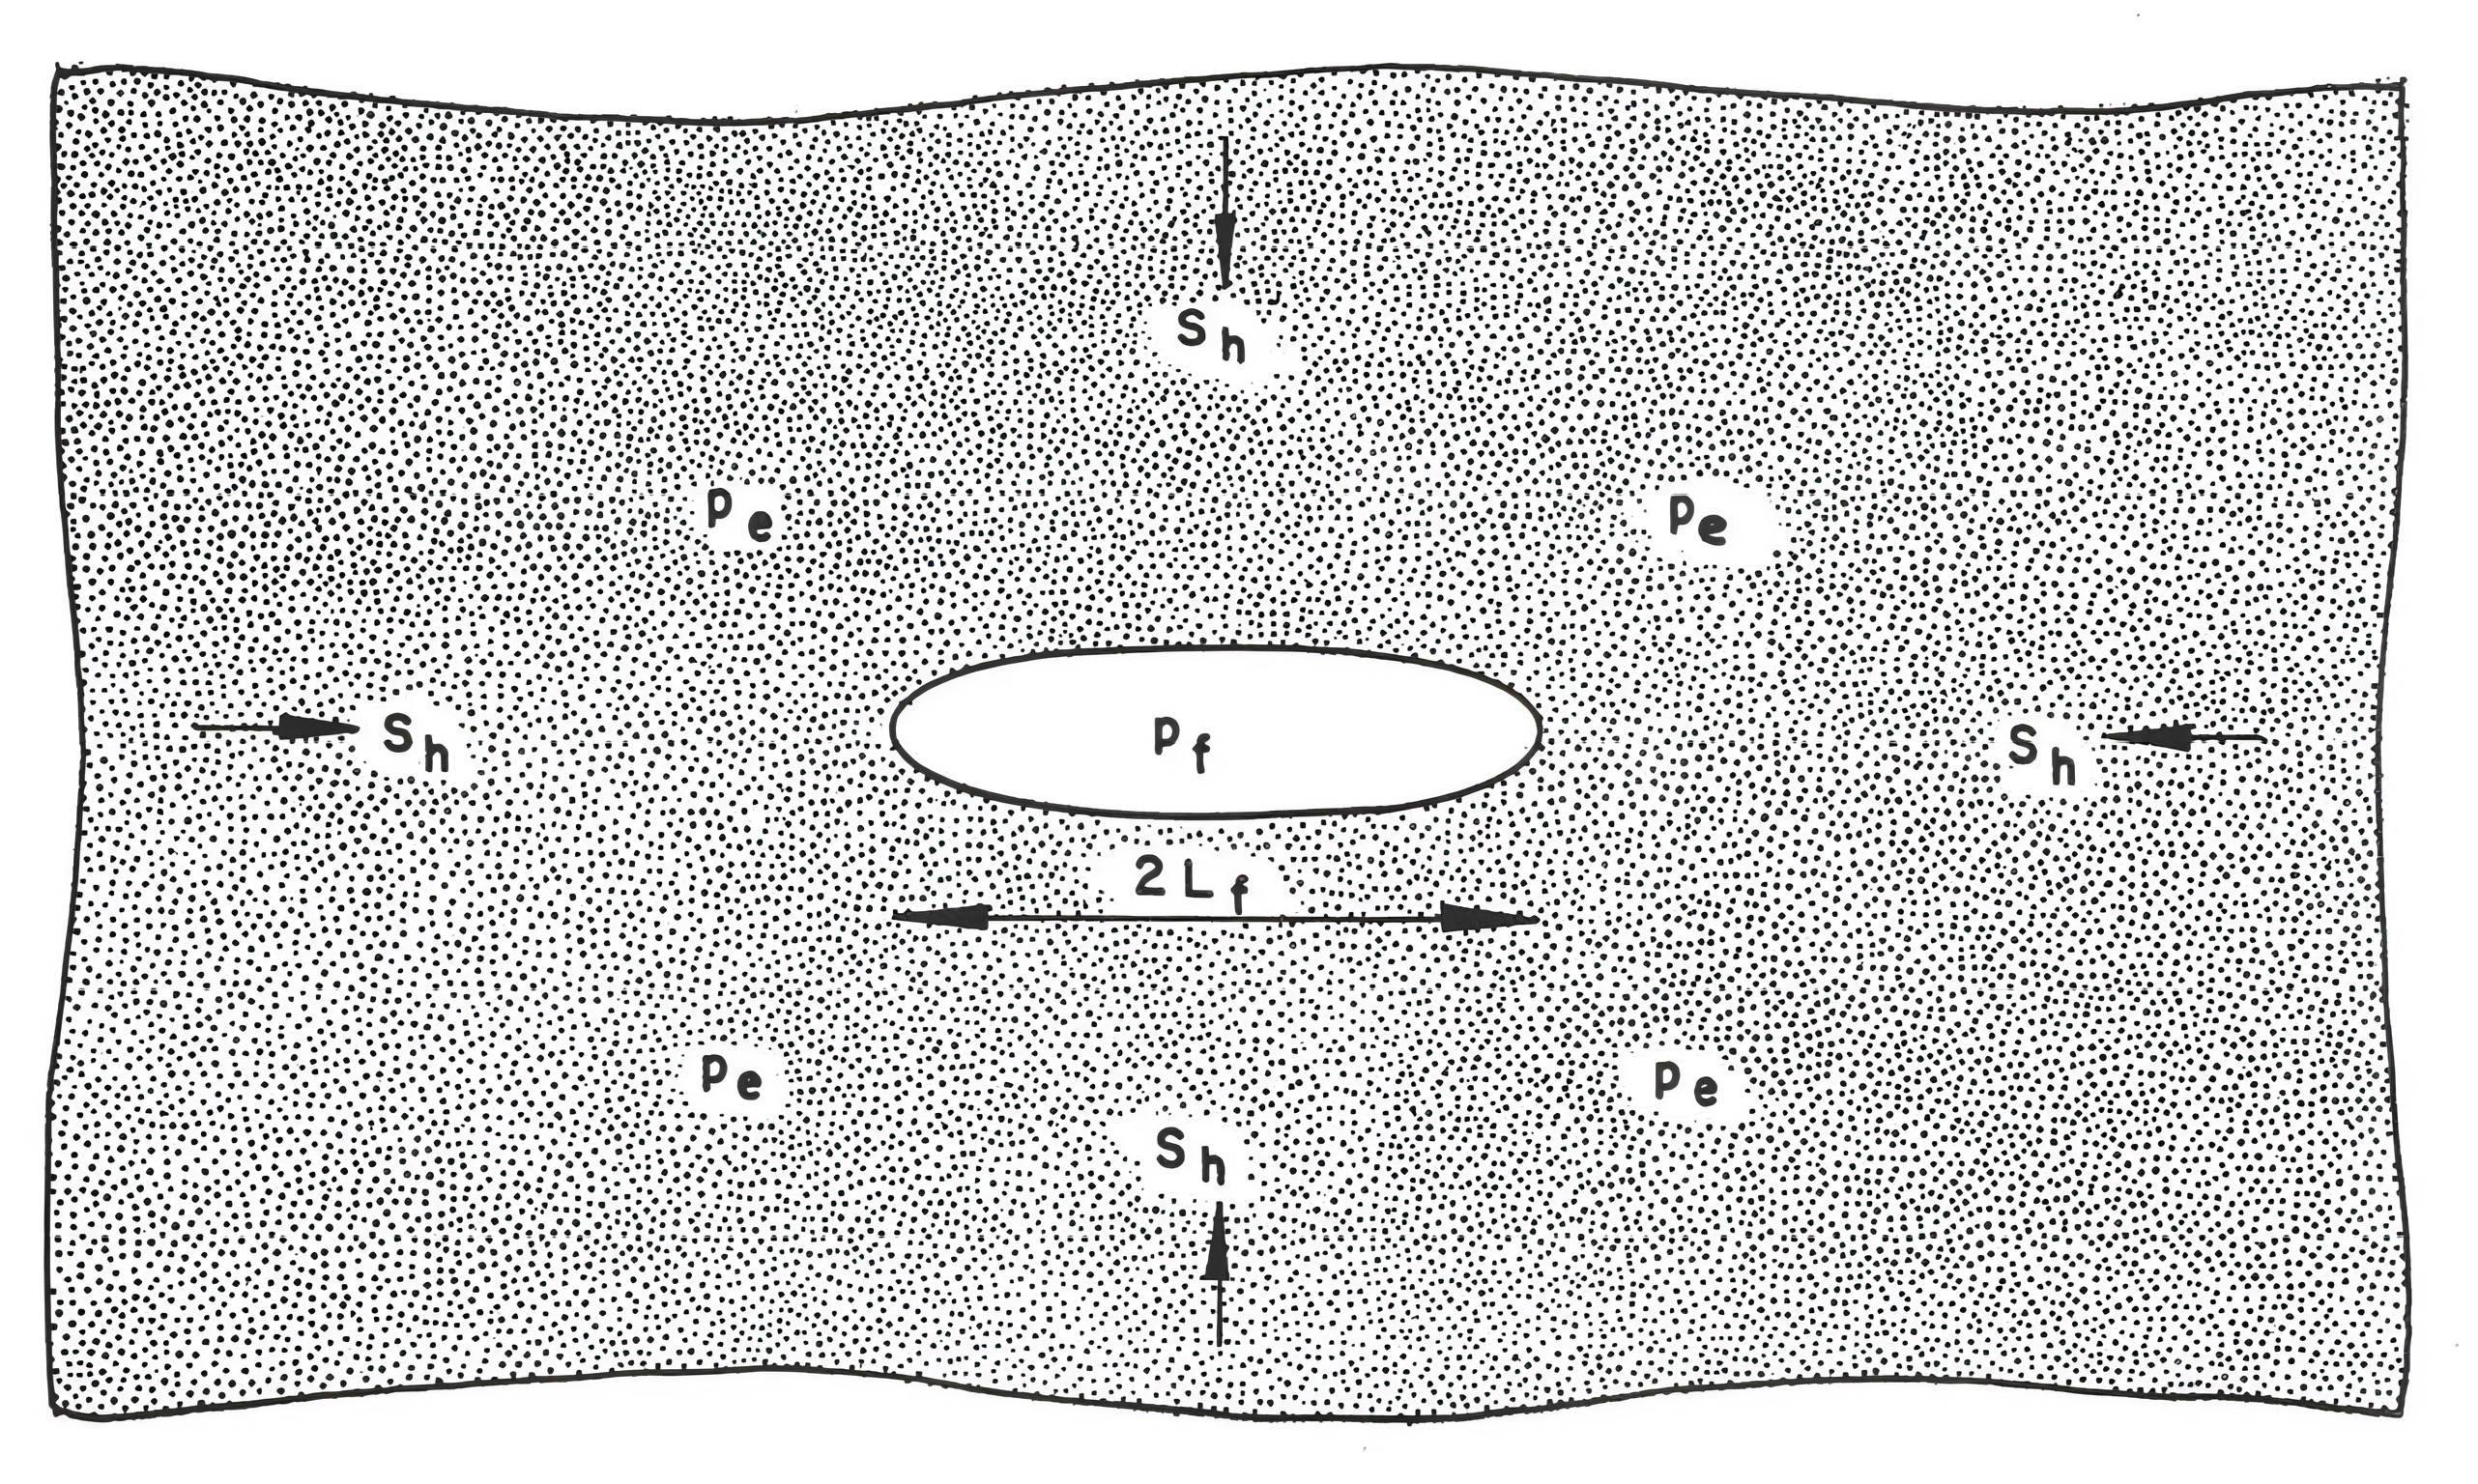
\includegraphics[width=.55\linewidth]{images/Hagoort_model_scheme.jpg}
\caption{KGD трещина в пороупругой породе \cite{hagoort_phd} (вид сверху; пренебрегаем вязкостью жидкости)} 
\label{fig:hagoort_model_scheme}  
\end{figure}

При выводе решения в работе \cite{hagoort_phd} рассматривается трещина с полудлиной $L_{\!f}$, распространяющаяся от нагнетательной скважины в пористой проницаемой породе (рис. \ref{fig:hagoort_model_scheme}).
Предполагается, что высота трещины много больше её длины, а давление по всей длине трещине одинаково и равно $p_{\!f}$, откуда вытекает эллиптичность горизонтального сечения трещины.
Другими словами, для рассматриваемой трещины используется модель KGD с пренебрежимо малой вязкостью закачиваемой жидкости.
Также предполагается, что напряжение, действующее на трещину со стороны породы, постоянно и равно $S_h$, а пластовое давление вдали от трещины равно $p_e$.

Чтобы решить задачу аналитически, вводится упрощённый профиль порового давления, напоминающий истинный профиль порового давления:
\beq
p(\xi)=p_e+\Delta p \exp{\!\left(-\frac{\xi-\xi_f}{\lambda}\right)},
\eeq
где $\xi$ -- координата в эллиптической системе координат;
$\Delta p=p_f-p_e$ -- репрессия на пласт;
$\lambda$ -- константа темпа падения.

\begin{figure}[H] 
\center
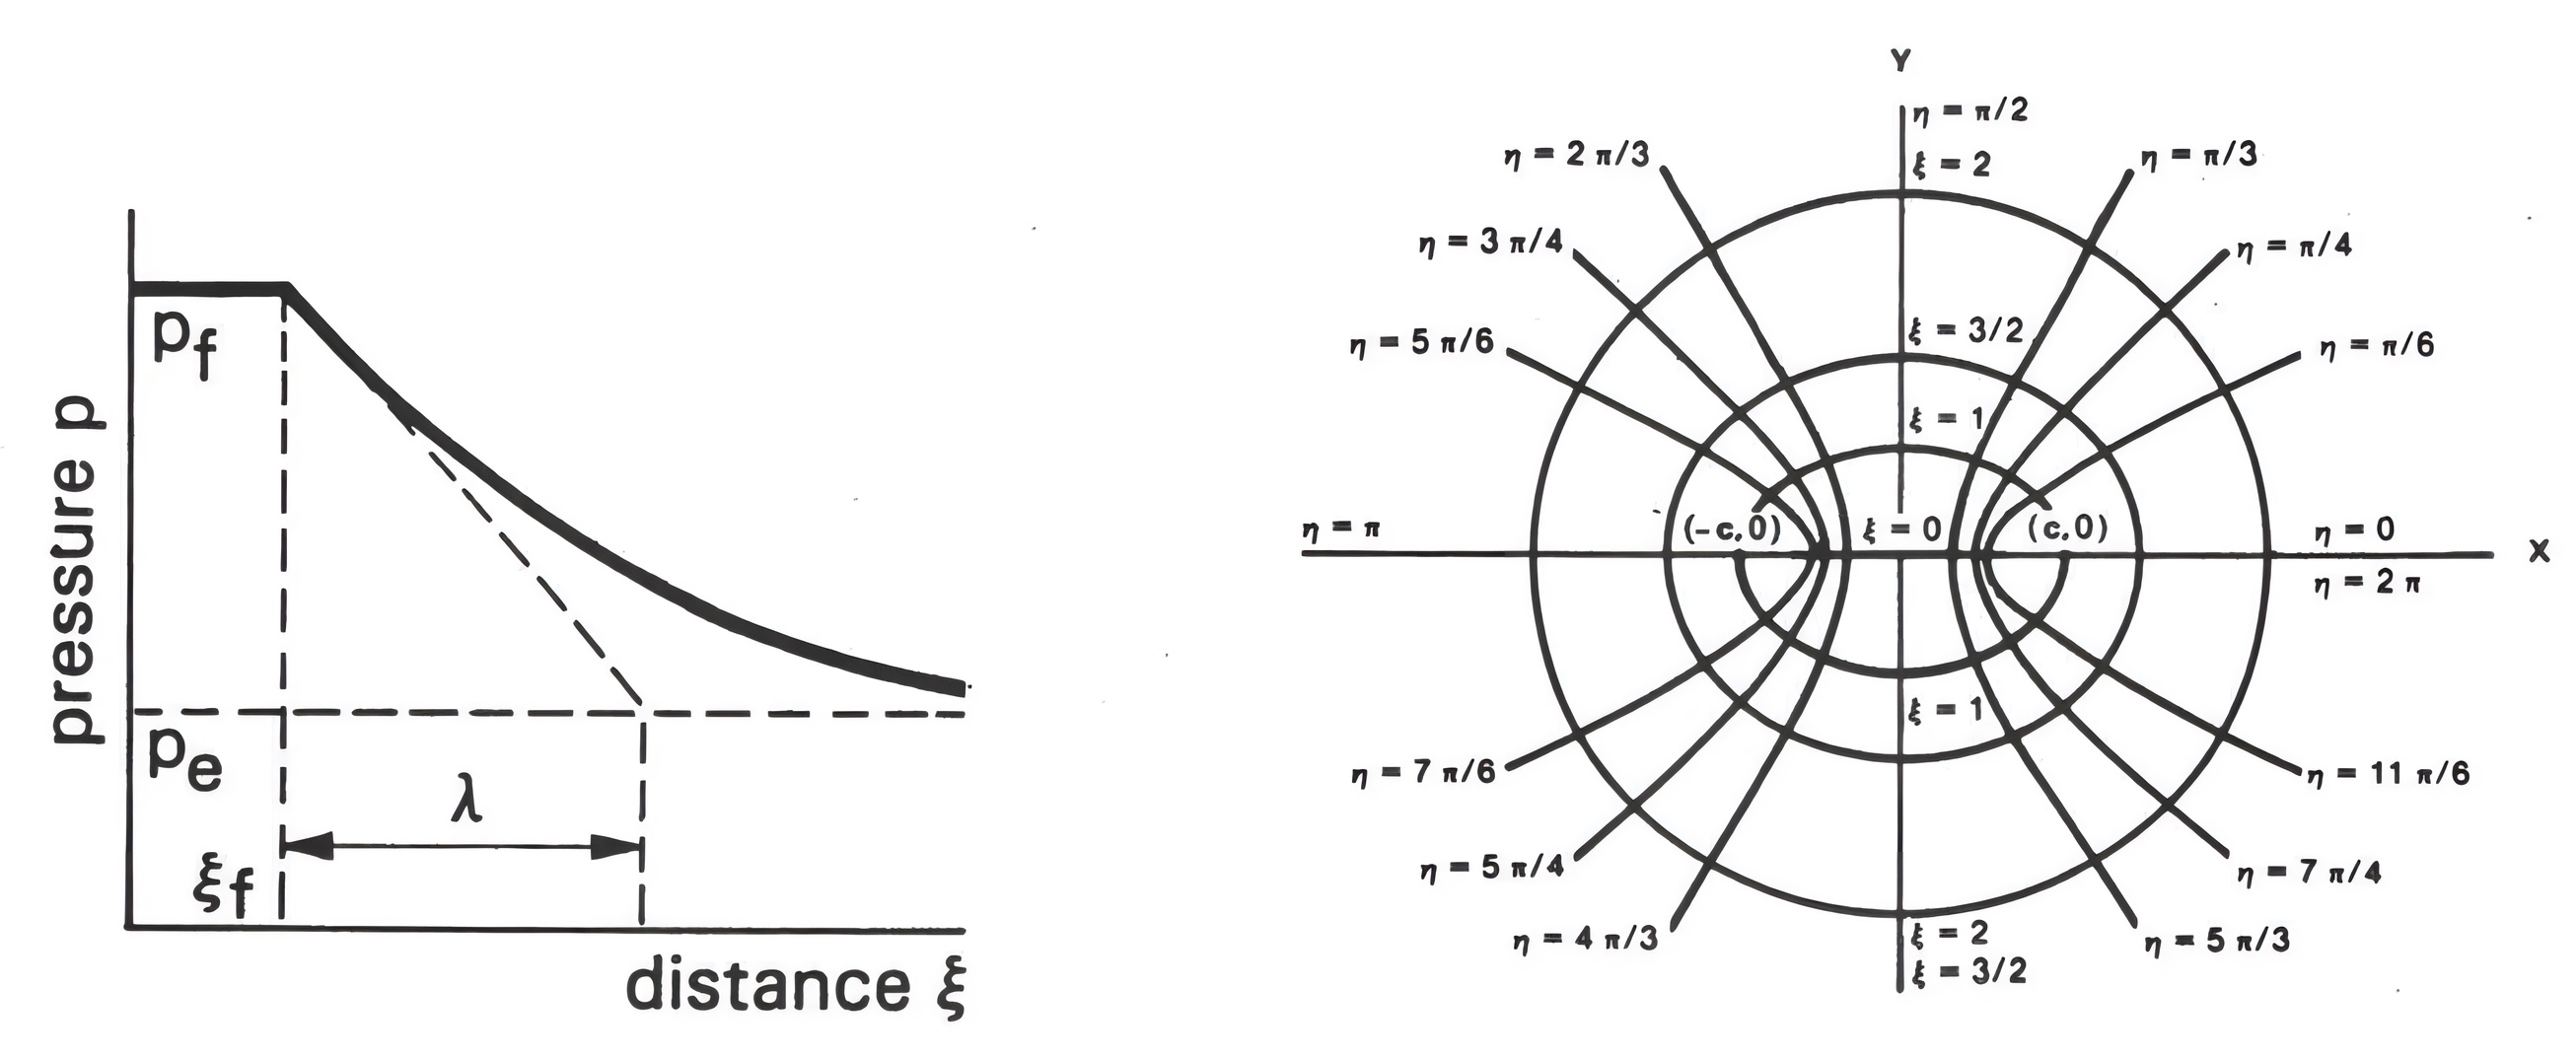
\includegraphics[width=\linewidth]{images/Hagoort_pressure_distribution.jpg}
\caption{Профиль порового давления (слева) и эллиптическая система координат (справа) \cite{hagoort_phd}} 
\label{fig:hagoort_pressure_distribution}  
\end{figure}

Этот профиль давления изображён на рис. \ref{fig:hagoort_pressure_distribution} и удовлетворяет граничным условиям на скважине ($p=p_f$) и на бесконечности ($p=p_e$).
Глубина проникновения давления определяется постоянной темпа падения $\lambda$, которую можно рассматривать как функцию времени.
Зависимость между глубиной проникновения давления $L_p$ и константой $\lambda$ задана в следующем виде:
\beq\label{Lp_via_lambda}
L_p=L_{\!f}\sinh{\lambda}
\eeq
При $\lambda\ll 1$ выражение \eqref{Lp_via_lambda} запишется в виде $L_p=\lambda L_f$, а при $\lambda\gg 1$ выражение \eqref{Lp_via_lambda} примет следующий вид: $\lambda=\ln{\left(2L_p/L_{\!f}\right)}$.

Распределение напряжений вокруг трещины найдено в виде суммы трёх функций упругих напряжений и специальной функции пороупругих напряжений.
На основе результатов, описанных в работе \cite{timoshenko_goodier}, и найденного распределения напряжений получено выражение для раскрытия трещины:
\beq\label{HaggoortFractureOpening}
u(x)=\frac{2\left(1-\nu^2\right)L_{\!f}\sqrt{1-\dfrac{x^2}{L_{\!f}^2}}}{E}\left(p_{\!f}-S_h-\frac{\lambda}{1+2\lambda}A\left(p_{\!f}-p_e\right)\right),
\eeq
где
$A=\dfrac{1-2\nu}{1-\nu}\left(1-\dfrac{c_r}{c_b}\right)$ -- пороупругая константа;
$c_r$ -- сжимаемость материала породы;
$c_b$ -- сжимаемость породы, насыщенной флюидами.

Максимальное раскрытие трещины (вблизи скважины) запишется в виде:
\beq
w_{\!f}=\frac{2\left(1-\nu^2\right)L_{\!f}}{E}\left(p_{\!f}-S_h-\frac{\lambda}{1+2\lambda}A\left(p_{\!f}-p_e\right)\right)
\eeq
Видим, что ширина трещины уменьшается при увеличении глубины проникновения давления.

Также из \eqref{HaggoortFractureOpening} вытекает формула для давления открытия/закрытия трещины ($u=0$):
\beq\label{HaggoortOpenCrit}
p_{\!f\!oc}=\dfrac{S_h-\dfrac{\lambda}{1+2\lambda}Ap_e}{1-\dfrac{\lambda}{1+2\lambda}A}
\eeq
Согласно \eqref{HaggoortOpenCrit} давление открытия/закрытия трещины увеличивается при увеличении глубины проникновения давления.
А при малых значениях $\lambda$ давление закрытия (оно же давление смыкания) трещины равно напряжению, действующему на трещину со стороны породы $p_{\!f\!oc}=S_h$.

Далее с помощью метода Гриффитса \cite{griffith} найдено давление распространения трещины:
\beq\label{HagoortProp}
p_{\!f\!p}=p_{\!f\!oc}+\frac{K_{Ic}/\sqrt{\pi L_{\!f}}}{\left(1-\dfrac{\lambda}{1+2\lambda}A\right)},
\eeq
где $K_{Ic}$ -- критический коэффициент интенсивности напряжений (трещиностойкость породы).

Таким образом, трещина остаётся стабильной (не распространяется), если давление в трещине выше давления открытия/закрытия трещины не более, чем на
$$
\frac{K_{Ic}/\sqrt{\pi L_{\!f}}}{\left(1-\dfrac{\lambda}{1+2\lambda}A\right)}.
$$
Это максимальное избыточное давление уменьшается при увеличении длины трещины (для длинных трещин давление распространения практически равно давлению смыкания) и увеличивается при увеличении глубины проникновения давления.

Однако, стоит ещё раз отметить, что формула для давления распространения трещины \eqref{HagoortProp} выведена только для трещин, у которых высота намного больше длины (модель KGD).
В работе \cite{kabanova_shel} получено выражение для давления распространения трещины в случае, когда её длина намного больше высоты (модель PKN), что больше соответствует действительности.

\section{Влияние модели утечек жидкости на моделирование роста трещин}
\vspace*{-5mm}

Важное исследование распространения трещин автоГРП было представлено в работе \cite{hagoort}, в которой путём совмещения аналитической модели трещины с численной моделью пласта изучена скорость распространения трещин.
В этой работе сделан вывод, что предположение одномерности утечек (модель Картера \cite{karter}) часто приводит к ошибочным результатам.

\begin{figure}[H] 
\center
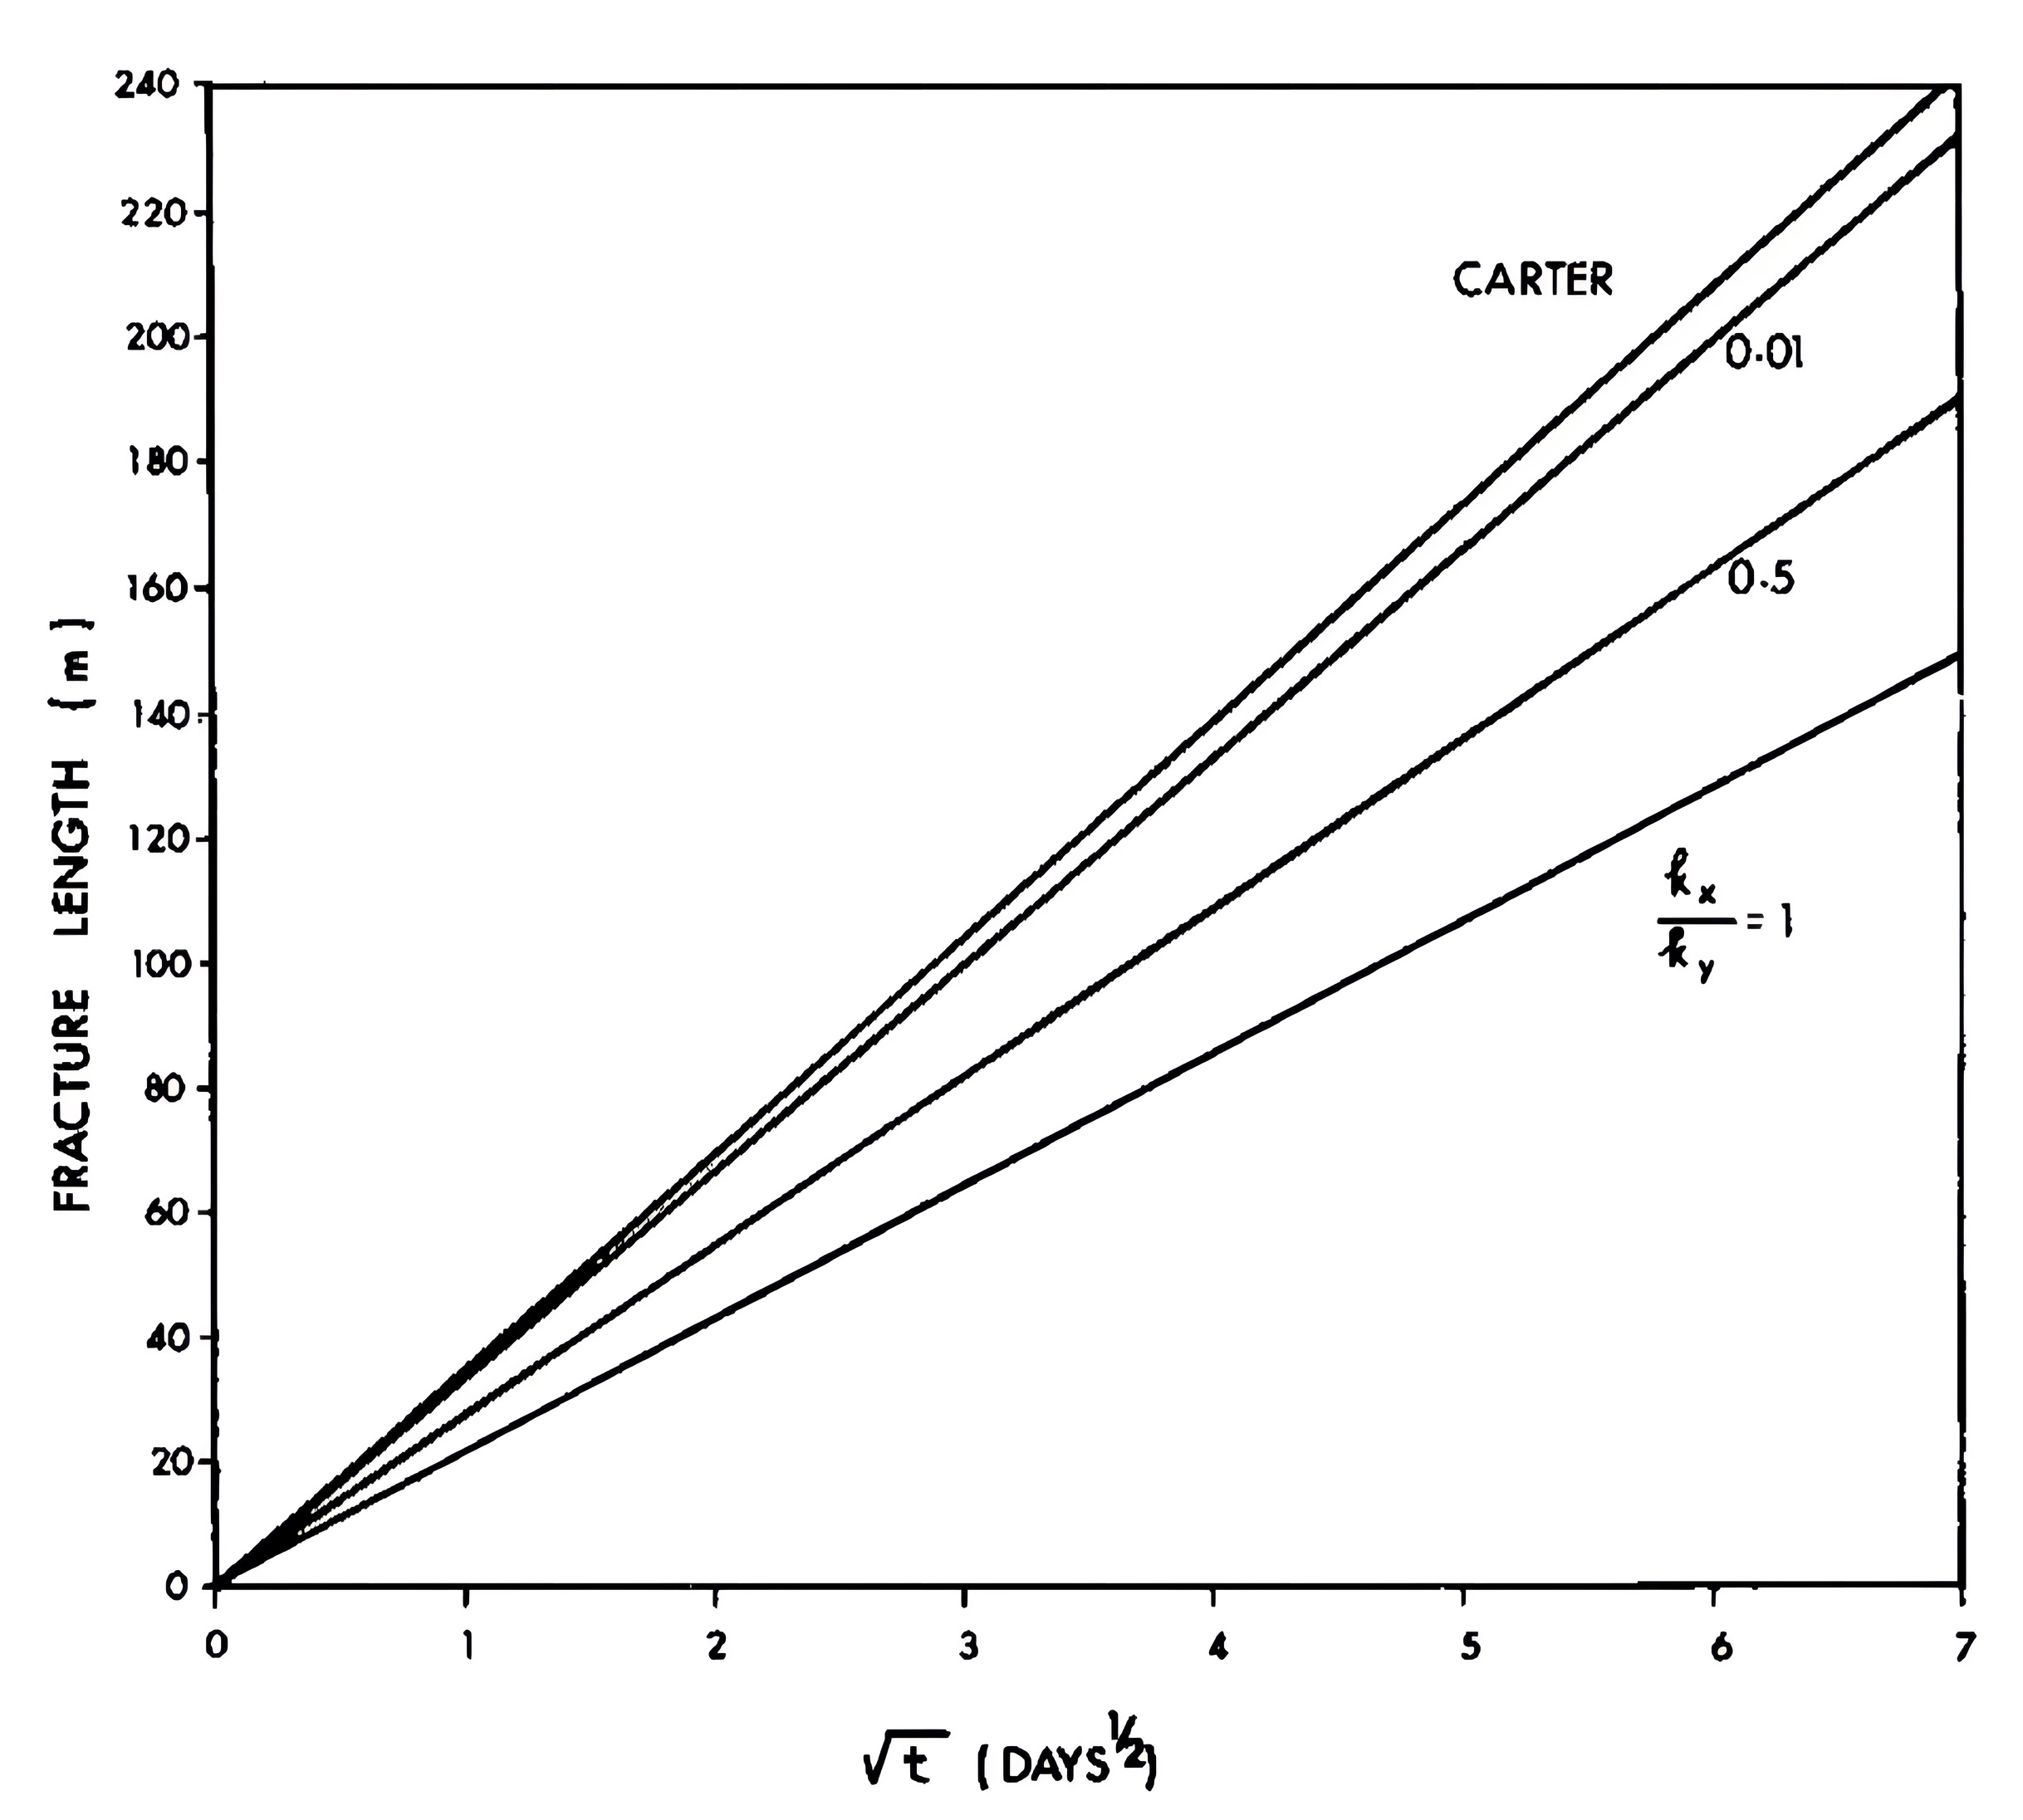
\includegraphics[width=.55\linewidth]{images/carter_vs_2D_leak_off.jpg}
\caption{Сравнение решения в режиме Картера с численным решением, полученным при различных значениях параметра анизотропии $k_x/k_y$ \cite{hagoort}} 
\label{fig:carter_vs_2D_leak_off}  
\end{figure}

А именно было проведено сравнение решения в режиме Картера с численным решением, которое было получено при различных значениях параметра анизотропии проницаемости $k_x/k_y$ (с помощью изменения анизотропии проницаемости осуществлялось управление направлением утечек -- при $k_x\ll k_y$ утечки одномерны и направлены перпендикулярно трещине, а при $k_x\approx k_y$ утечки двумерны).
Из рис. \ref{fig:carter_vs_2D_leak_off} видим, что использование предположения об одномерности утечек приводит к завышенным значениям длины трещины.

Позже в работе \cite{perkins_gonzalez} представлена модель распространения одной трещины автоГРП, в которой учтены двумерность утечек и влияние термоупругих изменений на скорость распространения трещин.
Было показано, что охлаждение породы вследствие закачки холодной воды может привести к очень длинным трещинам, так как при охлаждении порода сжимается и происходит термоупругое уменьшение горизонтальных напряжений пласта.

\section{Подход Кёнинга}
\vspace*{-5mm}

В статье Кёнинга \cite{koning} предложена модель трещины автоГРП, которая может включать как одномерные утечки, перпендикулярные трещине, так и двумерные радиальные утечки.

Показано, что если скорость распространения трещины существенно выше скорости распространения возмущения пластового давления, то применима модель одномерных утечек Картера \cite{karter}, перпендикулярных трещине.
В этом случае получено выражение для полудлины трещины автоГРП:
\beq\label{Koning1}
x_{\!f}=\frac{Q\mu\sqrt{\pi\kappa t}}{2\pi k_e h\left(p_{\!f}-p_e\right)},
\eeq
где $Q$ -- расход нагнетаемой в рассматриваемую трещину жидкости;
$\mu$ -- вязкость жидкости;
$\kappa=k_e/(\varphi_e\mu c_t)$ -- коэффициент пьезопроводности пласта;
$t$ -- время закачки;
$k_e$ -- проницаемость пласта;
$\varphi_e$ -- пористость пласта;
$c_t$ -- общая сжимаемость системы (состоит из сжимаемости флюидов и сжимаемости порового пространства);
$h$ -- эффективная толщина (мощность) пласта;
$\Delta p=p_{\!f}-p_e$ -- разница между средним давлением в трещине и пластовым давлением; $x_f$ -- полудлина трещины.

Если же трещина распространяется существенно медленнее возмущения пластового давления, то модель утечек Картера несомненно неприменима и требуется рассматривать более сложные модели утечек, например, двумерные радиальные утечки.
В этом случае в статье \cite{koning} также получена формула для полудлины трещины автоГРП:
\beq\label{Koning2}
x_{\!f}=3\exp{\left(-\frac{2\pi k_e h\left(p_{\!f}-p_e\right)}{Q\mu}\right)}\sqrt{\kappa t}
\eeq

В текущей работе для моделирования роста нескольких трещин автоГРП будут использованы формулы \eqref{Koning1} и \eqref{Koning2} из статьи Кёнинга \cite{koning}.

Однако в этих формулах есть зависимость полудлины трещины от расхода на трещине и репрессии на пласт, то есть от величин, значения которых могут изменяться со временем при росте трещин автоГРП, что затрудняет прямое использование формул \eqref{Koning1} и \eqref{Koning2} для расчёта полудлины трещины.

Основными причинами изменения расхода на трещине автоГРП являются изменение расхода на забое скважины и перераспределение потоков между трещинами (например, вследствие ухудшения качества перфораций на одной из трещин).
В следующей главе будет реализован алгоритм расчёта потоков (расходов) на каждой из нескольких трещин автоГРП при заданных входных параметрах, определяющих текущее физическое состояние породы, скважины и трещин.




